\documentclass[a4paper]{article}

\usepackage[utf8]{inputenc}
\usepackage[spanish,es-tabla]{babel}
\usepackage[T1]{fontenc}
\usepackage{microtype}
\usepackage{newspaper}
\usepackage{multicol}

%%\usepackage{url}
%%\usepackage{hyperref}
%%\usepackage{xcolor}
%%\hypersetup{
%%    colorlinks,
%%    linkcolor={red!50!black},
%%    citecolor={blue!50!black},
%%    urlcolor={blue!80!black}
%%}

%% ============================================================================
%% Referencias
%% ============================================================================
\usepackage[
	backend=biber,
	style=nejm,
]{biblatex}
\let\cite=\supercite %% Hace que las referencias aparezcan como superíndices
\addbibresource{referencias.bib} %% Añade el documento con referencias bibtex
\renewcommand*{\bibfont}{\footnotesize} %% Reduce el tamaño de fuente de las referencias

%% ============================================================================
%% Viñetas
%% ============================================================================
\usepackage[many]{tcolorbox}
\newtcolorbox{boxClinica}{
	sharpish corners, % better drop shadow
	boxrule = 0pt,
	toprule = 1.5pt, % top rule weight
	enhanced,
	fuzzy shadow = {0pt}{-2pt}{-0.5pt}{0.5pt}{black!35} % {xshift}{yshift}{offset}{step}{options} 
}

%% ============================================================================
%% Imágenes
%% ============================================================================
\usepackage{float}
\usepackage{graphicx}
\usepackage{wrapfig}
\usepackage{caption}
\captionsetup[figure]{font=footnotesize}

%% ============================================================================
%% Cabecera
%% ============================================================================
\date{\today}
\currentvolume{1}
\currentissue{1}
\SetPaperName{Gaceta Galénica}
\SetHeaderName{Gaceta Galénica}
\SetPaperLocation{Ciudad de Panamá}
\SetPaperSlogan{''Ciencia y Verdad.''}
\SetPaperPrice{SU-PMMV}

\newcommand{\NewsAuthor}[1]{%
	\hfill Por \textsc{#1} \vspace{4pt}
	\par \normalfont}	

%% 
\usepackage{newspaper-mod}
%%
\renewcommand{\headlinestyle}{\itshape\Large\lsstyle}
% \renewcommand{\bylinestyle}{\bfseries\Large\raggedright}
%%

%%%%%%%%%  Front matter   %%%%%%%%%%

\begin{document}

\maketitle

\begin{multicols}{3}


\byline{La Gaceta Galénica}{Moisés Serrano Samudio}

La Gaceta Galénica nace en esta primera edición como una publicación mensual de la coordinación de docencia de la Policlínica Lic. Manuel María Valdés. Es nuestro interés lanzar una edición el primer miércoles de cada mes con temas cortos dirigidos a mantener actualizados a los colegas médicos que desempeñan sus funciones en los distintos servicios de urgencias médico quirúrgicas en instalaciones de primer y segundo nivel de atención en Panamá.

Se publicará como un boletín digital informativo corto, de una a dos páginas de extensión, que enlazará a una versión web futura, permitiendo así a nuestros lectores ahondar en los temas expuestos. El tema central de la publicación se presentará como una viñeta clínica, a partir del cual se presentarán de manera práctica los aspectos fundamentados en medicina basada en evidencia más actualizados.

Planeamos incluir cápsulas históricas sobre la medicina en Panamá y repasar temas de bioestadística y epidemiología para ofrecer a nuestros lectores herramientas para refrescar la lectura crítica de la literatura médico-científica.

Sin mas preámbulo, esperamos que disfruten de su lectura tanto como nosotros disfrutamos preparando el contenido. Feliz lectura.

\closearticle


\headline{¿Quién fue Manuel María Valdés?}

Abogado, economista y periodista. Nace en 1907, proveniente de una familia de destacados juristas en el ámbito nacional de los primeros cincuenta años de la República de Panamá.

\begin{wrapfigure}{R}{0.18\textwidth}
	\begin{center}
		\vspace{-25pt}
		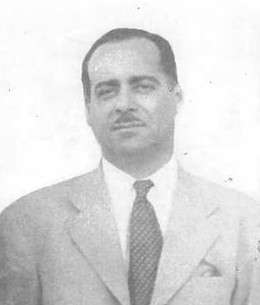
\includegraphics[width=0.17\textwidth]{mmvaldes.jpg}
	\end{center}
	\caption*{Lic. Manuel María Valdés}
\end{wrapfigure}

Al Lcdo. Manuel María Valdés, debemos el honor de la creación de la Caja de Seguro Social. La gesta que llevo a la fundación de la institución máxima de la seguridad social en Panamá, tuvo sus albores en 1937 en una reunión en París de Arnulfo Arias Madrid y Manuel María Valdés donde intercambiaban opiniones sobre seguros obligatorios\cite{Pinock95}.

Es la habilidad política junto a la orientación técnica de Don Manuel María Valdés y la tracción del Partido Liberal Unido lo que lleva a manos del Presidente Arnulfo Arias Madrid en 1941 a la firma de la Ley 23 del 21 de marzo de ese año, publicada en la Gaceta Oficial No. 8481 de marzo de 1941\cite{Pinock95},\cite{gaceta1941}.

Fundador de tres diarios: <<El Día>>, <<La Hora>> y <<El Mundo>>. Destacan en su producción bibliográfica, dos obras: Panamá y su soberanía monetaria (1951), Intervenciones electorales en Panamá (1932)\cite{Leonard15}.

Fallece en 1968, luego de toda una prolífica carrera. Apodado de cariño Nen, por sus familiares, amigos, conocidos y sus discípulos del periodismo. Es despedido en noviembre de ese año\cite{Lot68}.

\closearticle


\headline{Fibrilación atrial: Diagnóstico y manejo}

La fibrilación atrial es una patología que se ve con regular frecuencia en los servicios de urgencias. En mayores de 65 años tiene una incidencia de cerca del 10\% y se asocia a una serie de comorbilidades y predispone al desarrollo de patologías de gran morbimortalidad\cite{brundel_atrial_2022}.

\begin{boxClinica}

Paciente masculino de 64 años acude al servicio de urgencias por historia de palpitaciones, mareos, debilidad y diaforético. Sus signos vitales son: PA 160/106 mmHg, FC 131 lpm, FR 21 cpm, SpO2 95\%.

\end{boxClinica}

\closearticle

\printbibliography[heading=none]

\end{multicols}

\end{document}
